\documentclass[11pt,a4paper]{article}

% ---------------------------------------------------------------------------
% Packages
% ---------------------------------------------------------------------------
\usepackage[utf8]{inputenc}
\usepackage[T1]{fontenc}
\usepackage{lmodern}
\usepackage[margin=2.6cm]{geometry}
\usepackage{amsmath,amssymb,amsfonts}
\usepackage{graphicx}
\usepackage{xcolor}
\usepackage{booktabs}
\usepackage{multirow}
\usepackage{array}
\usepackage{caption}
\usepackage{subcaption}
\usepackage{enumitem}
\usepackage{float}
\usepackage{listings}
\usepackage{tikz}
\usetikzlibrary{positioning,arrows.meta,calc,shapes.geometric,decorations.pathreplacing,fit}
\usepackage{hyperref}
\hypersetup{colorlinks=true,linkcolor=blue!50!black,citecolor=blue!50!black,urlcolor=blue!50!black}
\usepackage[labelfont=bf]{caption}

% ---------------------------------------------------------------------------
% TODO / placeholder / review-note helpers
% ---------------------------------------------------------------------------
\newcommand{\todored}[1]{{\color{red}\textbf{[TODO: #1]}}}
\newcommand{\tbd}{{\color{red}\textbf{TBD}}}
% Generic red review note, not tied to a person
\newcommand{\rednote}[1]{{\color{red}\textbf{[NOTE: #1]}}}
% Red note addressed to a specific collaborator, e.g. \noteto{Tiago}{please check this}
\newcommand{\noteto}[2]{{\color{red}\textbf{[Note for #1: #2]}}}

\newcommand{\placeholderfig}[3]{%
% #1 width, #2 height (cm), #3 caption text describing what to insert
\begin{figure}[H]
\centering
\pgfmathsetmacro{\phw}{#1}
\pgfmathsetmacro{\phh}{#2}
\pgfmathsetmacro{\phtw}{#1-1}
\begin{tikzpicture}
\definecolor{phbg}{RGB}{250,240,240}
\draw[fill=phbg,draw=red!70!black,thick] (0,0) rectangle (\phw,\phh);
\draw[red!70!black,thick] (0,0) -- (\phw,\phh);
\draw[red!70!black,thick] (0,\phh) -- (\phw,0);
\node[align=center,text width=\phtw cm,text=red!70!black] at (\phw/2,\phh/2) {\small\textbf{PLACEHOLDER}\\[2pt]\footnotesize #3};
\end{tikzpicture}
\caption{\todored{#3}}
\end{figure}%
}

% ---------------------------------------------------------------------------
\title{\textbf{Lily}: System Design, Guidance and Control of an\\ Autonomous Surface Vehicle}
\author{Francisco \\ \todored{Course name, institution and instructor -- fill in}}
\date{\today}

\begin{document}

\maketitle

\begin{abstract}
This report documents the system architecture, actuation calibration, control, guidance and simulation stack developed for \textit{Lily}, a differential-thrust Autonomous Surface Vehicle (ASV). We describe the vehicle's physical configuration and state estimation pipeline, the in-water calibration of the propulsion system, the decoupled surge/yaw PID velocity controller and its thruster mixing, an Integral Line-Of-Sight (ILOS) trajectory-following law, the GPS-waypoint mission-management layer, and the Gazebo-based digital twin used for development and validation. Experimental results for velocity tracking and trajectory-following performance are reported in Section~\ref{sec:results}. \todored{Add one or two sentences to the abstract once the Results section is filled in with real numbers.}
\end{abstract}

\tableofcontents
\newpage

% =============================================================================
\section{The System}
\label{sec:system}
% =============================================================================

\textit{Lily} is a twin-thruster (differential-thrust) unmanned surface vehicle developed for autonomous survey and cooperative deploy/retrieve missions. The vehicle is controlled by a companion computer running ROS~2, bridged to a MAVLink autopilot (via \texttt{mavros}) that handles low-level attitude/position estimation, and interfaces with two brushless thrusters through VESC electronic speed controllers (ESCs) operating in Field-Oriented Control (FOC) mode.

\begin{figure}[ht!]
    \centering
    \includegraphics[width=\textwidth]{figures/bright_photo.jpg}
    \caption{The Lily USV, a twin-thruster autonomous surface vehicle.}
    \label{fig:lily}
\end{figure}

\subsection{Vehicle configuration and thruster layout}
\label{sec:hull}

The vehicle frame defines the sensor and actuator mounting points relative to \texttt{base\_link}, summarized in Table~\ref{tab:frames} and Figure~\ref{fig:layout}.

\begin{table}[H]
\centering
\caption{Sensor and actuator mounting offsets relative to \texttt{base\_link} (meters).}
\label{tab:frames}
\begin{tabular}{@{}llccc@{}}
\toprule
Frame & Component & $x$ [m] & $y$ [m] & $z$ [m] \\
\midrule
\texttt{left\_engine\_link}  & Port thruster      & $-0.80$ & $+0.33$ & $-0.15$ \\
\texttt{right\_engine\_link} & Starboard thruster & $-0.80$ & $-0.33$ & $-0.15$ \\
\texttt{lidar\_sensor}       & 3D LiDAR           & $+1.00$ & $0.00$  & $+0.70$ \\
\texttt{camera\_sensor}      & Monocular camera   & $+1.20$ & $0.00$  & $+0.70$ \\
\bottomrule
\end{tabular}
\end{table}

The two thrusters are mounted symmetrically about the centerline at the stern, giving a thruster (skid-steer) baseline of
\begin{equation}
L \;=\; y_{\text{left}} - y_{\text{right}} \;=\; 0.33 - (-0.33) \;=\; 0.66\ \text{m},
\end{equation}
which is exactly the \texttt{wheel\_base} parameter ($0.66$~m) used throughout the control stack (Section~\ref{sec:vw}). \todored{Confirm overall hull length/beam/draft and dry mass -- the URDF only encodes frame offsets, not the hull geometry. The velocity-controller comment in \texttt{velocity\_controller\_real.yaml} notes an estimated mass $\approx 42$\,kg and yaw inertia $I_z \approx 26\,\text{kg}\,\text{m}^2$; confirm/replace with measured values.}

\begin{figure}[H]
\centering
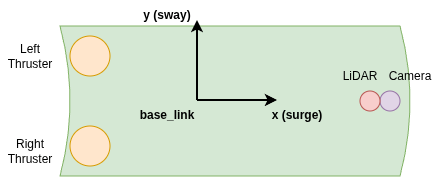
\includegraphics[width=0.7\textwidth]{figures/esquema.drawio.png}
\caption{Vehicle layout and sensor/actuator mounting points.}
\label{fig:layout}
\end{figure}

\subsection{Compute and communications architecture}

Figure~\ref{fig:arch} shows the software architecture. The companion computer runs ROS~2 nodes for guidance, control and perception; \texttt{mavros} bridges MAVLink telemetry commands to and from the autopilot; the autopilot performs attitude and position estimation and redirects RC input, arming and mode services.

\begin{figure}[H]
\centering
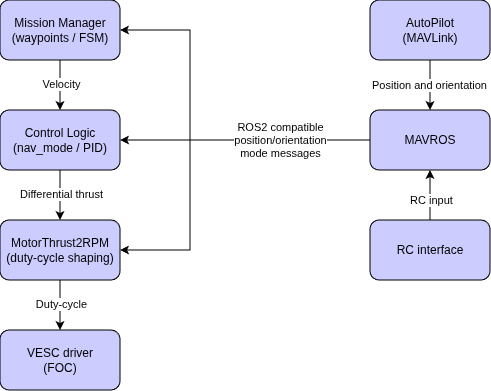
\includegraphics[width=0.7\textwidth]{figures/esquema2.drawio.png}
\caption{Software architecture.}
\label{fig:arch}
\end{figure}

\subsection{Localization and State Estimation}
\label{sec:localization}

The vehicle's pose and velocity feedback, used by all high-level control systems, rely on an Extended Kalman Filter (EKF) running natively on the autopilot's onboard firmware. Rather than computing state estimates within the external companion computer workspace, the higher-level control architecture acts purely as a consumer of the autopilot's telemetry. 

The onboard EKF operates as a black-box state estimator, fusing two primary sensor streams:
\begin{itemize}
    \item \textbf{High-rate Inertial Measurement Unit (IMU) data:} Providing angular rate and linear acceleration. For this 3~DoF Unmanned Surface Vehicle (USV), the critical components are planar accelerations and yaw rate. 
    \item \textbf{Global Navigation Satellite System (GNSS/GPS) data:} Supplying raw global positioning fixes.
\end{itemize}

By fusing these inputs, the EKF produces a stabilized, continuous odometry signal containing the vehicle's fused pose and velocity (twist). This finalized estimate is the sole feedback signal driving the vehicle's control logic, velocity regulation, and mission management. 

To map the global GPS data into a usable Cartesian space for 3~DoF planar control, a local East-North-Up (ENU) datum is established at the beginning of each operational session. In simulation environments, this origin is automatically parsed from the simulated world's configuration, whereas on the physical vehicle, it is initialized by the autopilot upon arming. Once this local datum is set, the mission manager converts all global geodetic waypoints (latitude and longitude) into local ENU coordinates using a flat-Earth approximation. This allows the USV to navigate using standard planar geometry relative to its starting location.

\begin{center}
\rednote{Should we dive into the EKF formulation (state vector, prediction/correction equations), or just describe that we used the ArduSub/ArduPilot on-board EKF as-is, without re-deriving it here?}
\end{center}

\todored{Confirm which autopilot firmware and EKF (e.g. ArduPilot EKF3, PX4 EKF2) Lily actually runs, and, if we do decide to elaborate, paste in the actual noise/process covariance tuning (\texttt{EK3\_*} or \texttt{EKF2\_*} parameters) so the description is vehicle-specific rather than generic.}

% =============================================================================
\section{Motor Calibration}
\label{sec:motor}
% =============================================================================

\begin{center}
\noteto{Tiago}{Please review this whole motor calibration section -- check whether the description of the thrust-shaping, dead-band, ramp and FOC logic below is still accurate and consistent with the current code (\texttt{motor\_thrust2RPM}, VESC configs), and flag anything we should add, correct, or cut before this goes in the report.}
\end{center}

Thrust commands travel through three stages before becoming water flow, as sketched in Figure~\ref{fig:actuation}: (i)~\texttt{ControlLogic}/\texttt{VelocityController} compute a desired thrust in Newtons per side; (ii)~\texttt{motor\_thrust2RPM} converts that thrust command into a bounded, rate-limited ESC duty cycle; (iii)~the VESC driver forwards the duty cycle to the ESC, which runs closed-loop FOC commutation on the BLDC thruster motor.

\begin{figure}[H]
\centering
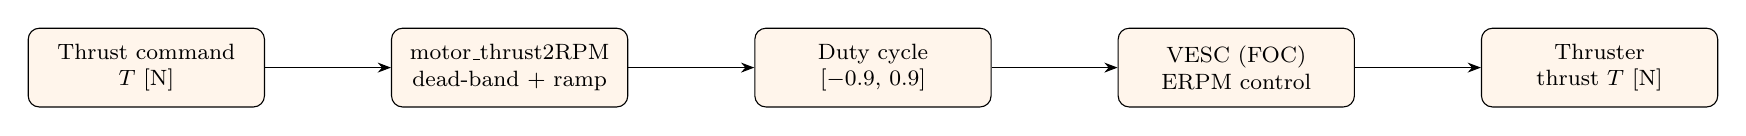
\begin{tikzpicture}[>=Stealth,node distance=6mm,every node/.style={font=\footnotesize}]
\tikzstyle{blk}=[draw,rounded corners,fill=orange!8,minimum width=3.0cm,minimum height=1.0cm,align=center]
\node[blk] (a) {Thrust command\\$T$ [N]};
\node[blk,right=16mm of a] (b) {motor\_thrust2RPM\\dead-band + ramp};
\node[blk,right=16mm of b] (c) {Duty cycle\\$[-0.9,\,0.9]$};
\node[blk,right=16mm of c] (d) {VESC (FOC)\\ERPM control};
\node[blk,right=16mm of d] (e) {Thruster\\thrust $T$ [N]};
\draw[->] (a)--(b); \draw[->] (b)--(c); \draw[->] (c)--(d); \draw[->] (d)--(e);
\end{tikzpicture}
\caption{Actuation chain from commanded thrust to delivered thrust.}
\label{fig:actuation}
\end{figure}

\subsection{Thrust-to-duty-cycle shaping (\texttt{motor\_thrust2RPM})}

The node first normalizes the requested thrust by the configured \texttt{max\_thrust}:
\begin{equation}
d_{\text{target}} = \frac{T_{\text{cmd}}}{T_{\max}}, \qquad d_{\text{target}} \in [-1,1].
\end{equation}
A dead-band suppresses commands too small to overcome static friction/cogging:
\begin{equation}
d_{\text{target}} = 0 \quad \text{if} \quad |d_{\text{target}}| < d_{\text{base}}, \qquad d_{\text{base}} = 0.08.
\end{equation}
The duty cycle is then rate-limited so the propeller never receives a step input. Three ramp modes are implemented; the deployed configuration uses \textbf{mode 2 (quadratic ease-out)}, in which the allowed rate of change grows quadratically with the remaining error, giving a soft start and a snappy finish:
\begin{align}
e_{\text{ramp}} &= \frac{|d_{\text{target}} - d_{\text{last}}|}{d_{\max}}, \quad \text{clamped to } [0,1] \\
\dot d_{\text{allowed}} &= \underbrace{0.2\, \dot d_{\max}}_{\text{base rate}} \;+\; \underbrace{20\, \dot d_{\max}}_{\text{explosive rate}} \cdot e_{\text{ramp}}^2, \\
\Delta d_{\max} &= \dot d_{\text{allowed}} \cdot \Delta t, \\
d_{\text{last}} &\leftarrow d_{\text{last}} + \operatorname{clamp}(d_{\text{target}}-d_{\text{last}},\,-\Delta d_{\max},\,\Delta d_{\max}),
\end{align}
where $\dot d_{\max}=$ \texttt{max\_duty\_cycle\_rate} $=0.9\,\text{s}^{-1}$. A zero-crossing (sign reversal of the command) triggers an instantaneous stop-before-reverse when \texttt{instant\_deceleration=true}, modeling the fact that water drag decelerates the hull quickly compared to thruster spin-up; same-direction deceleration is smoothed if \texttt{smooth\_same\_dir\_decel=true}. The result is clipped to $d\in[d_{\min},d_{\max}]=[-0.9,\,0.9]$ before being published as the duty-cycle command.

\begin{table}[H]
\centering
\caption{\texttt{motor\_thrust2RPM} parameters (identical for sim and real, \texttt{lily\_control/cfg/*.yaml}).}
\label{tab:t2rpm}
\begin{tabular}{@{}lcl@{}}
\toprule
Parameter & Value & Meaning \\
\midrule
\texttt{max\_duty\_cycle} / \texttt{min\_duty\_cycle} & $\pm 0.9$ & Saturation limits \\
\texttt{max\_duty\_cycle\_rate} & $0.9\,\text{s}^{-1}$ & Max slew of duty cycle \\
\texttt{ramp\_mode} & 2 (quadratic) & 0 none / 1 linear / 2 quadratic ease-out \\
\texttt{base\_duty\_cycle} & 0.08 & Static-friction dead-band \\
\texttt{startup\_thresh} & 0.10 & Reduced accel. below this target (mode 1) \\
\texttt{instant\_deceleration} & true & Snap to zero on direction reversal \\
\texttt{smooth\_same\_dir\_decel} & true & Ramp (not snap) when slowing without reversing \\
\texttt{loop\_rate} & 50\,Hz & Node update rate \\
\bottomrule
\end{tabular}
\end{table}

\subsection{VESC configuration and FOC commutation}

The duty-cycle command is sent over a serial link (\texttt{transport\_drivers/serial\_driver}) to a VESC-based ESC running in Field-Oriented Control mode. Table~\ref{tab:vesc} lists the deployed limits (\texttt{vesc/vesc\_driver/params/vesc\_config.yaml}).

\begin{table}[H]
\centering
\caption{VESC configuration limits.}
\label{tab:vesc}
\begin{tabular}{@{}lc@{}}
\toprule
Parameter & Value \\
\midrule
Serial port & \texttt{/dev/ttyACM0} \\
Duty cycle range & $[-1.0,\,1.0]$ (driver clamps to $\pm0.9$ upstream) \\
Motor current limit & $[0,\,100]$\,A \\
Speed limit (ERPM) & $\pm 23250$ \\
Brake current range & $[-20000,\,200000]$ \\
Servo output range & $[0.15,\,0.85]$ \\
\bottomrule
\end{tabular}
\end{table}

FOC commutation requires an in-water motor detection/calibration pass so that winding resistance, inductance and flux-linkage (and, if used, encoder/Hall offset) are identified under realistic load -- a submerged propeller presents a very different load curve than the motor spinning in air. \todored{Describe here the exact FOC detection procedure you ran in water (VESC ``Motor FOC $\rightarrow$ Detect'' wizard values: measured resistance, inductance, flux linkage $\lambda$, and any manual current/KV overrides), and the resulting current/torque constants ($K_t$, $K_v$) that were applied.}

\subsection{Thrust curve (ERPM $\rightarrow$ thrust)}
\label{sec:thrustcurve}

The relationship between commanded electrical RPM (ERPM) and delivered thrust is modeled with the standard quadratic propeller law (thrust $\propto n^2$ for fixed pitch, fixed advance ratio):
\begin{equation}
T(\text{erpm}) \;=\; T_{\max}\left(\frac{\text{erpm}}{\text{erpm}_{\max}}\right)^{2},
\label{eq:thrustcurve}
\end{equation}
with the reference values used to generate the calibration table (\texttt{vesc\_driver/scripts/motor\_curve.py}): $\text{erpm}_{\max}=23300$ (matching the VESC \texttt{speed\_max}$\,\approx 23250$ configured above) and $T_{\max}=200\,\text{N}$. This curve is what the FOC controller's closed-loop speed regulation and the thrust$\to$duty-cycle node above are calibrated against.

\begin{figure}[H]
\centering
\begin{tikzpicture}
\begin{scope}
\draw[->] (0,0) -- (7.2,0) node[right]{\footnotesize ERPM};
\draw[->] (0,0) -- (0,4.4) node[above]{\footnotesize Thrust [N]};
\draw[domain=0:7,samples=60,thick,blue] plot ({\x},{4*(\x/7)*(\x/7)});
\node at (3.5,-0.6) {\footnotesize $\text{erpm}_{\max}=23300$};
\node at (-1.1,4.1) {\footnotesize $T_{\max}=200$~N};
\draw[dashed,gray] (7,0) -- (7,4);
\draw[dashed,gray] (0,4) -- (7,4);
\end{scope}
\end{tikzpicture}
\caption{Nominal quadratic thrust curve, Eq.~\eqref{eq:thrustcurve}, used as the calibration reference.}
\label{fig:thrustcurve}
\end{figure}

\todored{This is the nominal/assumed quadratic model, not a fit to logged bench or in-water force-gauge data. If a real static-thrust-stand or in-water bollard-pull test was performed, insert the measured (erpm, thrust) data points here, refit Eq.~\eqref{eq:thrustcurve} (or a more general polynomial) against them, and report the fit residuals.}

% =============================================================================
\section{Vehicle Dynamics}
\label{sec:dynamics}
% =============================================================================

\begin{center}
\noteto{Diogo}{Could you work on this section a bit? The idea is a short, more mechanical/physics-oriented treatment of Lily's vehicle dynamics (rigid-body equations of motion, added mass, hydrodynamic damping, etc.) to complement the control-oriented surge/yaw model in Section~\ref{sec:vw}. Feel free to pull from the marine/robot-vehicle-dynamics class notes -- a standard 3-DOF (surge, sway, yaw) surface-vehicle model (e.g.\ Fossen-style $M\dot\nu + C(\nu)\nu + D(\nu)\nu = \tau$) would fit well here. Doesn't need to be long, just enough to justify the simplified model used later in the report.}
\end{center}

This section is intended to give a brief, physics-first description of the rigid-body and hydrodynamic effects governing Lily's motion in the horizontal plane, before Section~\ref{sec:vw} simplifies this down to the decoupled surge/yaw model actually used by the controller.

\todored{Placeholder -- add: (i) the 3-DOF rigid-body equations of motion in body-fixed coordinates; (ii) added-mass and hydrodynamic damping terms relevant to a planar USV hull; (iii) any simplifying assumptions (e.g.\ neglecting sway/roll authority) that justify the decoupled surge/yaw model used in Section~\ref{sec:vw}.}

% =============================================================================
\section{$v$/$w$ Control: Kinematics and PID Design}
\label{sec:vw}
% =============================================================================

\begin{center}
\noteto{Francisco}{Please look into this section and add supporting pictures/screenshots (e.g.\ real thruster mixing test, PID step-response plots from bench/pool tests, autotuner limit-cycle capture) wherever useful.}
\end{center}

\subsection{Body-frame kinematics}

Lily is modeled as a planar, differential-thrust (skid-steered) surface vehicle. Let $v$ denote surge (forward) speed and $w$ the yaw rate, both expressed in the body frame and measured from the fused odometry (\texttt{odom.twist.twist.linear.x}, \texttt{odom.twist.twist.angular.z}). Ignoring sway (no side-thruster authority) the rigid-body equations of motion are
\begin{align}
m\,\dot v  &= F_{\text{surge}} - d_v(v)\,v, \label{eq:surgeeom}\\
I_z\,\dot w &= M_{\text{yaw}} - d_w(w)\,w, \label{eq:yaweom}
\end{align}
with $m\approx 42$\,kg, $I_z \approx 26\ \text{kg}\,\text{m}^2$ (per the controller configuration comments -- \todored{replace with measured mass/inertia}), and $d_v(\cdot)$, $d_w(\cdot)$ lumped (possibly speed-dependent) hydrodynamic drag terms that are not modeled explicitly -- instead, their effect is compensated for by the feedback PID controller of Section~\ref{sec:pid} and identified indirectly through relay-based autotuning (Section~\ref{sec:autotune}). See Section~\ref{sec:dynamics} for a more complete treatment of the underlying vehicle dynamics.

\subsection{Thruster mixing}
\label{sec:mixing}

The two collinear, aft-mounted thrusters can only produce a surge force and a yaw moment about \texttt{base\_link} (no direct sway or roll authority):
\begin{align}
F_{\text{surge}} &= T_{\text{left}} + T_{\text{right}}, \\
M_{\text{yaw}} &= (T_{\text{right}} - T_{\text{left}})\cdot \frac{L}{2}, \qquad L = 0.66\ \text{m (wheel\_base)}.
\end{align}
Inverting this $2\times2$ linear mixer gives the thrust allocation actually implemented in \texttt{velocity\_controller.cpp}:
\begin{align}
T_{\text{left}}  &= \tfrac{1}{2}F_{\text{surge}} - \frac{M_{\text{yaw}}}{L}, \label{eq:mixL}\\
T_{\text{right}} &= \tfrac{1}{2}F_{\text{surge}} + \frac{M_{\text{yaw}}}{L}. \label{eq:mixR}
\end{align}
Both are subsequently clamped to $\pm T_{\max}$ (\texttt{max\_thrust}).

\subsection{Decoupled surge/yaw PID}
\label{sec:pid}

Surge and yaw are controlled by two independent PID loops running at $f_s=$\texttt{loop\_rate\_hz}$=50$\,Hz ($\Delta t = 1/f_s$), closing around the fused-odometry measurements $v_{\text{meas}}, w_{\text{meas}}$ against the commanded $v_{\text{cmd}}, w_{\text{cmd}}$ (from \texttt{/cmd\_vel}, itself produced either by the ILOS guidance law of Section~\ref{sec:ilos} or an operator teleop command):
\begin{align}
e_v[k] &= v_{\text{cmd}}[k] - v_{\text{meas}}[k], &
e_w[k] &= w_{\text{cmd}}[k] - w_{\text{meas}}[k].
\end{align}
The derivative term is computed \emph{on the measurement} rather than on the error, which avoids the classical ``derivative kick'' whenever the setpoint changes abruptly:
\begin{align}
\dot v_{\text{meas}}[k] &\approx -\frac{v_{\text{meas}}[k]-v_{\text{meas}}[k-1]}{\Delta t}, &
\dot w_{\text{meas}}[k] &\approx -\frac{w_{\text{meas}}[k]-w_{\text{meas}}[k-1]}{\Delta t}.
\end{align}
The PID outputs (a force and a moment, i.e.\ the gains carry physical units $\text{N}/(\text{m/s})$ and $\text{N}\!\cdot\!\text{m}/(\text{rad/s})$) are
\begin{align}
F_{\text{surge}}[k] &= k_{v,p}\,e_v[k] + k_{v,i}\,I_v[k] + k_{v,d}\,\dot v_{\text{meas}}[k], \label{eq:pidF}\\
M_{\text{yaw}}[k]   &= k_{w,p}\,e_w[k] + k_{w,i}\,I_w[k] + k_{w,d}\,\dot w_{\text{meas}}[k], \label{eq:pidM}
\end{align}
with integral states updated \emph{after} the tentative output is computed, using \emph{directional} anti-windup: the integral is only allowed to accumulate further in the direction that would deepen an already-saturated output; it may always unwind:
\begin{align}
I_v[k] &=
\begin{cases}
\operatorname{clamp}\!\big(I_v[k-1] + e_v[k]\Delta t,\; -I_{v,\max},\, I_{v,\max}\big) & \text{if not saturated, or } e_v[k]\cdot I_v[k-1] < 0\\
I_v[k-1] & \text{otherwise (blocked)}
\end{cases}
\end{align}
(analogously for $I_w$), where "saturated" means $|T_{\text{left}}|\!\geq\! T_{\max}$ or $|T_{\text{right}}|\!\geq\! T_{\max}$ \emph{after} mixing (Eqs.~\eqref{eq:mixL}--\eqref{eq:mixR}), and $I_{v,\max}=$\texttt{v\_int\_max}, $I_{w,\max}=$\texttt{w\_int\_max}. Finally $F_{\text{surge}}, M_{\text{yaw}}$ are mixed into $T_{\text{left}}, T_{\text{right}}$ and clamped to $\pm T_{\max}$.

A per-side slew-rate limiter (\texttt{SlewRateLimiter}, max rate \texttt{max\_thrust\_rate}) is applied to the final thrust commands \emph{after} mixing, in every control mode (including MANUAL and TELEOP), to protect the driveline from step commands:
\begin{equation}
T_{\text{side}}[k] = T_{\text{side}}[k-1] + \operatorname{clamp}\!\Big(T_{\text{side}}^{\text{cmd}}[k]-T_{\text{side}}[k-1],\, -\dot T_{\max}\Delta t,\ \dot T_{\max}\Delta t\Big).
\end{equation}

\begin{table}[H]
\centering
\caption{Decoupled PID gains, integral limits and slew rate (surge $v$ and yaw $w$).}
\label{tab:pid}
\begin{tabular}{@{}lcccccc@{}}
\toprule
Config & $k_{v,p}$ & $k_{v,i}$ & $k_{v,d}$ & $I_{v,\max}$ & $T_{\max}$ [N] & $\dot T_{\max}$ [N/s]\\
\midrule
Simulation (\texttt{velocity\_controller\_sim.yaml}) & 172.0 & 41.0 & 58.0 & 10.0 & 100 & 200 \\
Real vehicle (\texttt{velocity\_controller\_real.yaml}) & 50.0 & 20.0 & 40.0 & 1.0 & 100 & 100\\
\bottomrule
\end{tabular}
\vspace{4pt}
\begin{tabular}{@{}lcccc@{}}
\toprule
Config & $k_{w,p}$ & $k_{w,i}$ & $k_{w,d}$ & $I_{w,\max}$ \\
\midrule
Simulation & 660.0 & 300.0 & 40.0 & 10.0 \\
Real vehicle & 50.0 & 10.0 & 10.0 & 1.0 \\
\bottomrule
\end{tabular}
\end{table}

Both configurations share $L=0.66$\,m, $f_s=50$\,Hz, \texttt{cmd\_timeout}$=0.5$\,s (command watchdog: \texttt{/cmd\_vel} is zeroed if stale). \todored{The simulation gains were obtained from the adaptive relay autotuner (Section~\ref{sec:autotune}) and are noticeably higher than the hand-tuned real-vehicle gains -- re-run the autotuner on the real boat once in-water access is available and update this table with the resulting $K_u$, $T_u$ and final gains.}

\subsection{Relay-feedback PID autotuning}
\label{sec:autotune}

Both an offline (\texttt{relay\_autotuner.py}) and an adaptive online variant (\texttt{adaptive\_relay\_autotuner.py}) implement the classical \textbf{Åström--Hägglund relay-feedback method} to identify the plant's ultimate gain and period without needing an explicit dynamic model. The velocity PID is bypassed and a relay of amplitude $d$ drives $F_{\text{surge}}$ (surge test) or $M_{\text{yaw}}$ (yaw test, with a small constant forward force $F_f$ superimposed so the differential thruster pair retains authority) directly:
\begin{equation}
u(t) = d\cdot\operatorname{sign}\big(e(t)\big), \qquad e(t) = \text{setpoint} - \text{measurement},
\end{equation}
with hysteresis $\varepsilon$ on the sign decision to reject chatter. Under relay feedback the plant settles into a limit cycle of period $T_u$ and amplitude $a$. The describing function of an ideal relay is $N(a) = 4d/(\pi a)$; imposing the Barkhausen criterion $G(j\omega_u)N(a)=-1$ at the limit-cycle frequency $\omega_u = 2\pi/T_u$ gives the ultimate gain and period:
\begin{equation}
K_u = \frac{4d}{\pi a}, \qquad T_u = \text{measured oscillation period}.
\end{equation}
Convergence is declared once the coefficient of variation of amplitude and period over the most recent full cycles drops below a tolerance (5\% by default). Three tuning rules are implemented (Table~\ref{tab:tuningrules}); \textbf{Tyreus--Luyben} is the default, chosen for its lower overshoot ($\sim$15\%) on integrating, sluggish, marine-type plants compared to classical Ziegler--Nichols ($\sim$40\% overshoot):
\begin{align}
K_p &= K_u/3.2, & K_i &= \frac{K_p}{2.2\,T_u}, & K_d &= \frac{K_p\,T_u}{6.3}. &&\text{(Tyreus--Luyben)}
\end{align}

\begin{table}[H]
\centering
\caption{Relay-autotuner tuning rules implemented in \texttt{relay\_autotuner.py}.}
\label{tab:tuningrules}
\begin{tabular}{@{}lccc@{}}
\toprule
Rule & $K_p$ & $K_i$ & $K_d$ \\
\midrule
Tyreus--Luyben (default) & $K_u/3.2$ & $K_p/(2.2\,T_u)$ & $K_p T_u/6.3$ \\
Ziegler--Nichols (closed loop) & $0.6\,K_u$ & $K_p/(0.5\,T_u)$ & $0.125\,K_p T_u$ \\
Conservative (PI only) & $K_u/4.5$ & $K_p/(2.5\,T_u)$ & $0$ \\
\bottomrule
\end{tabular}
\end{table}

The \emph{adaptive} variant additionally re-tunes the relay amplitude $d$ and hysteresis $\varepsilon$ online between half-cycles: it increases $d$ if the limit-cycle amplitude is buried in the hysteresis band (weak signal), increases $\varepsilon$ if half-cycles are too short (chattering), decreases $d$ on over-excitation, and bumps $d$ upward if no zero-crossing is observed for longer than \texttt{stalled\_cycle\_warn\_sec} (stalled/unreachable setpoint) -- up to a bounded adaptation budget before aborting.

\todored{Insert the actual $K_u$, $T_u$, limit-cycle amplitude $a$ and resulting gains reported by the autotuner run(s) that produced Table~\ref{tab:pid}'s simulation gains, and (once available) the real-vehicle run.}

\subsection{Mode state machine}

\texttt{ControlLogic} is the sole owner of a 4-state mode machine (Figure~\ref{fig:fsm}) and the sole gate to the autopilot's \texttt{SetMode}/arming services; RC input always has final authority. \texttt{MissionManager} (Section~\ref{sec:mission}) never asserts a mode directly -- it requests \texttt{GUIDED}/\texttt{POSHOLD} through a service that \texttt{ControlLogic} may reject while RC override is active.

\begin{figure}[H]
\centering
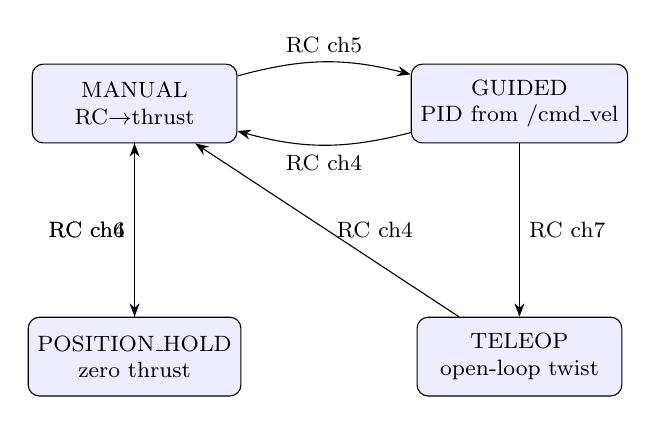
\begin{tikzpicture}[>=Stealth,node distance=22mm,every node/.style={font=\footnotesize}]
\tikzstyle{st}=[draw,rounded corners,fill=blue!7,minimum width=2.6cm,minimum height=1cm,align=center]
\node[st] (manual) {MANUAL\\RC$\to$thrust};
\node[st,right=of manual] (guided) {GUIDED\\PID from /cmd\_vel};
\node[st,below=of manual] (pos) {POSITION\_HOLD\\zero thrust};
\node[st,below=of guided] (teleop) {TELEOP\\open-loop twist};
\draw[->] (manual) to[bend left=15] node[above]{RC ch5} (guided);
\draw[->] (guided) to[bend left=15] node[below]{RC ch4} (manual);
\draw[->] (manual) -- node[left]{RC ch6} (pos);
\draw[->] (pos) -- node[left]{RC ch4} (manual);
\draw[->] (guided) -- node[right]{RC ch7} (teleop);
\draw[->] (teleop) -- node[right]{RC ch4} (manual);
\end{tikzpicture}
\caption{\texttt{ControlLogic} mode FSM. Edge-triggered RC channel thresholds ($>1600\,\mu\text{s}$) drive transitions; only a GUIDED $\to$ MANUAL/POSITION\_HOLD/TELEOP switch from RC is a hard override that blocks MissionManager's software requests.}
\label{fig:fsm}
\end{figure}

% =============================================================================
\section{Trajectory Following: Integral Line-Of-Sight (ILOS) Guidance}
\label{sec:ilos}
% =============================================================================

\begin{center}
\noteto{Francisco}{Please look into this section and add supporting pictures (e.g.\ logged path vs.\ ILOS guidance geometry overlay, real cross-track error traces) wherever useful.}
\end{center}

\subsection{Path-frame errors}

Given the current path leg from waypoint $\mathbf{p}=(p_x,p_y)$ to the next waypoint $\mathbf{t}=(t_x,t_y)$, the path-tangential angle is
\begin{equation}
\alpha_k = \operatorname{atan2}(t_y - p_y,\; t_x - p_x).
\end{equation}
Rotating the vehicle's position $\mathbf{c}=(c_x,c_y)$ relative to $\mathbf{p}$ into the path frame gives the along-track error $e_x$ (used for the lookahead point) and the cross-track error $e_y$ (the signed perpendicular distance to the path, positive to the left):
\begin{align}
e_x &= \cos\alpha_k\,(c_x-p_x) + \sin\alpha_k\,(c_y-p_y), \\
e_y &= -\sin\alpha_k\,(c_x-p_x) + \cos\alpha_k\,(c_y-p_y).
\end{align}

\subsection{Lookahead point and ILOS heading law}

A lookahead point is placed a fixed distance $\Delta$ (\texttt{lookahead\_distance}) ahead of the vehicle's along-track projection, clipped so it never overshoots the target waypoint:
\begin{equation}
s = \min\!\big(e_x + \Delta,\ \|\mathbf{t}-\mathbf{p}\|\big), \qquad \mathbf{\ell} = \mathbf{p} + s\,(\cos\alpha_k,\sin\alpha_k).
\end{equation}
Pure (proportional) LOS would steer the bow toward $\boldsymbol\ell$ using $\psi_d = \alpha_k + \arctan(-e_y/\Delta)$; this drives $e_y\to 0$ only in the absence of a constant disturbance (current, wind). To reject a constant environmental disturbance with zero steady-state cross-track error, an \emph{integral} term is added on the cross-track error (Integral-LOS, following Fossen \& Pettersen):
\begin{align}
\dot I_y &= e_y, \qquad I_y \leftarrow \operatorname{clamp}(I_y,\, -I_{y,\max},\, I_{y,\max}), \label{eq:ilosint}\\
\tilde e_y &= e_y + k_i\, I_y, \label{eq:ilosaug}\\
\psi_d &= \alpha_k + \arctan\!\left(\frac{-\tilde e_y}{\Delta_{\text{eff}}}\right), \qquad \Delta_{\text{eff}} = \max\big(0.1,\ \|\boldsymbol\ell - \mathbf{c}\|\big), \label{eq:iloslaw}\\
\psi_e &= \operatorname{wrap}_{(-\pi,\pi]}(\psi_d - \psi), \label{eq:heading_err}
\end{align}
where $k_i=$\texttt{ki\_los}, $I_{y,\max}=$\texttt{max\_integral\_e\_y}, and $\psi$ is the vehicle's current yaw. In the deployed mission configurations $k_i=0$ (Table~\ref{tab:ilosparams}), i.e. the integral action is wired in and available but currently disabled -- pure LOS is being used operationally. \todored{Decide whether to enable $k_i>0$ for missions with strong current/wind, and report the cross-track error improvement if you do.}

\subsection{Speed law}

Forward speed is commanded proportional to remaining distance, but is weighted down whenever the vehicle is not pointed at the lookahead point -- this is what prevents the ASV from surging sideways while turning onto a new leg -- and is decelerated inside an arrival radius so that the vehicle settles rather than overshoots each waypoint:
\begin{align}
d_{\text{tgt}} &= \|\mathbf{t}-\mathbf{c}\|, \\
\text{align} &= \begin{cases} \big(\max(0,\cos\psi_e)\big)^{n} & |\psi_e| < \psi_{\text{thr}} \\ 0 & \text{otherwise} \end{cases}, \qquad n = \texttt{align\_exponent}, \label{eq:align}\\
v_{\text{allow}} &= \begin{cases} \max\!\big(0.1,\ v_{\max}\, d_{\text{tgt}}/R_{\text{arr}}\big) & d_{\text{tgt}} < R_{\text{arr}} \\ v_{\max} & \text{otherwise} \end{cases}, \\
v_{\text{cmd}} &= \operatorname{clamp}\!\big(k_{p,\text{lin}}\, d_{\text{tgt}}\cdot\text{align},\ 0,\ v_{\text{allow}}\big), \\
w_{\text{cmd}} &= \operatorname{clamp}\!\big(k_{p,\text{ang}}\, \psi_e,\ -w_{\max},\ w_{\max}\big).
\end{align}
The waypoint is declared reached once $d_{\text{tgt}} < R_{\text{wp}}$ (\texttt{waypoint\_radius}), at which point the ILOS integrator is reset and the leg advances to the next waypoint pair.

\begin{figure}[H]
\centering
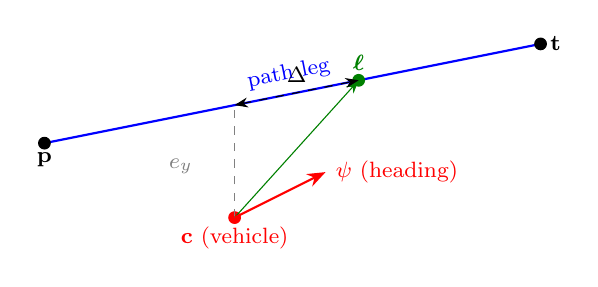
\begin{tikzpicture}[>=Stealth,scale=1.05]
\coordinate (p) at (0,0);
\coordinate (t) at (6,1.2);
\draw[thick,blue] (p) -- (t) node[midway,above,sloped]{\footnotesize path leg};
\filldraw (p) circle(2pt) node[below]{\footnotesize $\mathbf{p}$};
\filldraw (t) circle(2pt) node[right]{\footnotesize $\mathbf{t}$};
\coordinate (c) at (2.3,-0.9);
\filldraw[red] (c) circle(2pt) node[below]{\footnotesize $\mathbf{c}$ (vehicle)};
% projection foot
\coordinate (foot) at (2.3,0.46);
\draw[dashed,gray] (c) -- (foot);
\node[gray] at (1.65,-0.28) {\footnotesize $e_y$};
% lookahead point
\coordinate (l) at (3.8,0.76);
\filldraw[green!50!black] (l) circle(2pt) node[above]{\footnotesize $\boldsymbol\ell$};
\draw[green!50!black,->] (c) -- (l);
\draw[<->,dashed] (foot) -- (l) node[midway,above]{\footnotesize $\Delta$};
% heading
\draw[->,thick,red] (c) -- ++(1.1,0.55) node[right]{\footnotesize $\psi$ (heading)};
\end{tikzpicture}
\caption{ILOS guidance geometry: cross-track error $e_y$, lookahead distance $\Delta$, lookahead point $\boldsymbol\ell$, and desired heading $\psi_d$ toward $\boldsymbol\ell$ (Eq.~\eqref{eq:iloslaw}).}
\label{fig:ilos}
\end{figure}

\begin{table}[H]
\centering
\caption{ILOS/waypoint guidance parameters (\texttt{lily\_nav} mission configs).}
\label{tab:ilosparams}
\begin{tabular}{@{}lccc@{}}
\toprule
Parameter & Square mission & Viana buoys mission & Meaning\\
\midrule
$k_{p,\text{lin}}$ & 0.5 & 0.5 & Linear gain [1/s]\\
$k_{p,\text{ang}}$ & 1.5 & 1.5 & Angular gain [1/s]\\
$v_{\max}$ & 1.0 m/s & 0.5 m/s & Max commanded surge \\
$w_{\max}$ & 0.5 rad/s & 0.5 rad/s & Max commanded yaw rate\\
$R_{\text{wp}}$ (\texttt{waypoint\_radius}) & 3.0 m & 3.0 m & Waypoint arrival tolerance\\
$R_{\text{arr}}$ (\texttt{arrival\_radius}) & 5.0 m & 5.0 m & Deceleration radius\\
$n$ (\texttt{align\_exponent}) & 2.0 & 2.0 & Heading-alignment sharpness\\
$\psi_{\text{thr}}$ & $28.6^\circ$ & $28.6^\circ$ & Max heading err.\ for forward motion\\
$\Delta$ (\texttt{lookahead\_distance}) & 3.0 m & 3.0 m & ILOS lookahead \\
$k_i$ (\texttt{ki\_los}) & 0.0 & 0.0 & Integral gain (disabled)\\
$I_{y,\max}$ & 5.0 & 20.0 & Integral clamp \\
Guidance loop rate & 10 Hz & 10 Hz & \\
\bottomrule
\end{tabular}
\end{table}

\todored{A simpler bearing-only \texttt{WaypointController} (proportional heading law, no lookahead/integral term) also exists in the codebase as a baseline; MissionManager currently instantiates only the ILOS \texttt{LosController}. Mention in the report if the baseline was used for any A/B comparison.}

% =============================================================================
\section{Trajectory Generation from Waypoints: Mission Manager}
\label{sec:mission}
% =============================================================================

\subsection{GPS $\to$ local ENU conversion}
\label{sec:gps2enu}

All guidance math (Section~\ref{sec:ilos}) operates in a local, metric East-North-Up (ENU) frame, while missions are authored in geodetic coordinates (latitude/longitude). \texttt{MissionManager} converts every waypoint once, on receipt of the local datum $(\varphi_0,\lambda_0)$ (Section~\ref{sec:ekf}), using the same flat-Earth (equirectangular) approximation used throughout the stack (accurate for ranges $\lesssim 10$\,km):
\begin{align}
x &= (\lambda - \lambda_0)\,\cos(\varphi_0)\cdot k, \\
y &= (\varphi - \varphi_0)\cdot k, \qquad k = 111319.5\ \text{m/deg (ArduPilot constant} \approx R_\oplus\cdot\pi/180).
\end{align}
This gives \texttt{MissionManager} a sequence of local ENU waypoints, which is what is actually handed to the ILOS guidance law leg-by-leg (Section~\ref{sec:ilos}).

\subsection{Mission finite-state machine}

\texttt{MissionManager} sequences a deploy/retrieve-style mission as a 6-state FSM, shown in Figure~\ref{fig:missionfsm}, that advances from waypoint to waypoint and reacts to a small set of service calls and arrival events.

\begin{figure}[H]
\centering
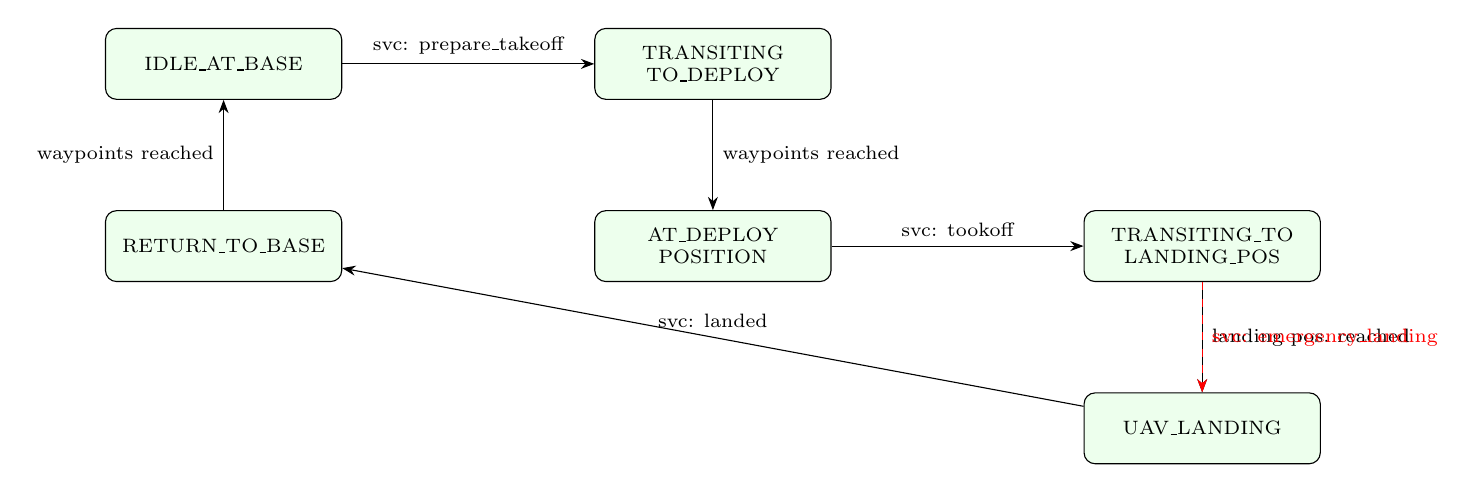
\begin{tikzpicture}[>=Stealth,node distance=14mm,every node/.style={font=\scriptsize}]
\tikzstyle{st}=[draw,rounded corners,fill=green!7,minimum width=3.0cm,minimum height=0.9cm,align=center]
\node[st] (idle) {IDLE\_AT\_BASE};
\node[st,right=32mm of idle] (deploy) {TRANSITING\\TO\_DEPLOY};
\node[st,below=of deploy] (atdeploy) {AT\_DEPLOY\\POSITION};
\node[st,below=of idle] (return) {RETURN\_TO\_BASE};
\node[st,right=32mm of atdeploy] (landtrans) {TRANSITING\_TO\\LANDING\_POS};
\node[st,below=of landtrans] (landing) {UAV\_LANDING};

\draw[->] (idle) -- node[above]{svc: prepare\_takeoff} (deploy);
\draw[->] (deploy) -- node[right]{waypoints reached} (atdeploy);
\draw[->] (atdeploy) -- node[above]{svc: tookoff} (landtrans);
\draw[->] (landtrans) -- node[right]{landing pos.\ reached} (landing);
\draw[->] (landing) -- node[above]{svc: landed} (return);
\draw[->] (return) -- node[left]{waypoints reached} (idle);
\draw[->,red,dashed] (landtrans) -- node[right,red]{svc: emergency\_landing} (landing);
\end{tikzpicture}
\caption{MissionManager finite-state machine: waypoints are consumed sequentially within each \texttt{TRANSITING\_*} leg, and the FSM advances once the leg's waypoints are reached or the corresponding service is called.}
\label{fig:missionfsm}
\end{figure}

\todored{Confirm/describe the cooperating UAV platform and CONOPS behind the deploy/retrieve service names (\texttt{prepare\_takeoff}, \texttt{tookoff}, \texttt{landed}, \texttt{emergency\_landing}), which indicate this mission profile was built for a cooperative USV$\to$UAV deploy/recovery operation.}

\subsection{Example missions}

Table~\ref{tab:missions} lists the two GPS mission definitions currently checked in, each specified as an ordered sequence of waypoints that \texttt{MissionManager} converts to ENU (Section~\ref{sec:gps2enu}) and feeds leg-by-leg to the ILOS guidance law.

\begin{table}[H]
\centering
\caption{Mission waypoint sets (WGS84 degrees).}
\label{tab:missions}
\begin{tabular}{@{}lll@{}}
\toprule
Mission & Leg & Waypoints (lat, lon) \\
\midrule
\multirow{3}{*}{Square (FEUP)} & Deploy & (41.685117, $-8.838916$) $\to$ (41.685399, $-8.839086$) $\to$ (41.685684, $-8.838855$)\\
 & Landing & (41.685399, $-8.839086$) \\
 & Return & (41.685117, $-8.838916$) \\
\midrule
\multirow{4}{*}{Viana buoys} & Deploy & (41.684793,$-8.839555$)$\to$(41.684922,$-8.839550$)$\to$(41.685022,$-8.839395$)\\
 & Deploy pos.\ & (41.685022, $-8.839395$)\\
 & Landing & (41.686183, $-8.839467$) \\
 & Return & reverse of deploy leg \\
\bottomrule
\end{tabular}
\end{table}

% =============================================================================
\section{Simulation Environment (\texttt{lily\_gz})}
\label{sec:sim}
% =============================================================================

\begin{center}
\noteto{Francisco}{This section please -- I've trimmed it down a lot: no need to get into ROS~2/bridging/topic-plumbing details here, that's covered structurally elsewhere. Focus this section on the Gazebo environment itself (worlds, assets) and the wave/wind plugins used to make it a realistic ASV testbed. Please also add pictures/screenshots of the simulated worlds and, if applicable, the wave/wind effects in action.}
\end{center}

\subsection{Overview}

The digital twin runs on \textbf{Gazebo Harmonic}, reusing several assets originally developed for VRX (the RobotX/VRX surface-vehicle simulation suite): buoys, docks, and land-block obstacles. \texttt{lily\_environment.launch.py} is config-driven -- it takes a \texttt{world} launch argument (e.g.\ \texttt{alqueva}, \texttt{viana}, \texttt{viana\_buoys}, \texttt{feup}, \texttt{empty}) and loads the corresponding \texttt{.sdf} world file, along with the models and per-world spawn poses that populate it.

\subsection{Environmental plugins: waves and wind}

\todored{Describe here the Gazebo plugins used to model the water surface (wave field: amplitude/period/direction, whether it produces visual-only waves or also hydrodynamic forcing on the hull) and wind (constant or gusting wind field, force/torque applied to the hull and any exposed superstructure). Note which worlds/missions had these environmental effects enabled versus running in calm/no-wind conditions, and whether the reported results (Section~\ref{sec:results}) were obtained with them on or off.}

\subsection{Vehicle model and worlds}

The \texttt{lily} Gazebo model (\texttt{lily\_gz/models/lily/model.sdf}) uses dedicated hull/housing/mount/propeller meshes and PBR textures. Five worlds are checked in: \texttt{empty} (unit testing), \texttt{feup} (campus pond, used for the square mission), \texttt{alqueva} and \texttt{viana}/\texttt{viana\_buoys} (larger reservoir/coastal environments, the latter with spawned red/dummy buoys for perception-in-the-loop testing), and \texttt{dynamic\_world} (\todored{describe the purpose of \texttt{dynamic\_world.sdf} -- e.g.\ moving obstacles/waves -- if used for the reported results}).

\begin{figure}[H]
\centering
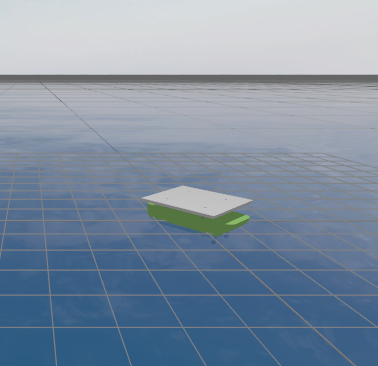
\includegraphics[width=0.6\linewidth]{figures/lily_gazebo.png}
\caption{The \texttt{lily} vehicle model floating in the Gazebo Harmonic simulation, showing the hull and deck meshes on the water surface.}
\label{fig:sim_world}
\end{figure}

% =============================================================================
\section{Results}
\label{sec:results}
% =============================================================================

\begin{center}
\noteto{Francisco}{This section is yours too -- please fill in the real logs/plots/numbers below once available (from pool/lake/field tests or simulation runs), and add the actual figures in place of the placeholders.}
\end{center}

This section reports closed-loop performance for (i) the decoupled $v$/$w$ velocity controller (Section~\ref{sec:vw}) in isolation, and (ii) the full ILOS trajectory-following stack (Section~\ref{sec:ilos}--\ref{sec:mission}) on the example missions of Table~\ref{tab:missions}. \todored{All figures and numeric values in this section are placeholders. Replace each placeholder box with the corresponding plot (e.g.\ exported from a rosbag via \texttt{rqt\_plot}/\texttt{plotjuggler}/matplotlib) and fill in the tables once logs from the pool/lake/field tests (or simulation runs) are available.}

\subsection{$v$/$w$ tracking performance}

\textbf{Test protocol.} The velocity controller was exercised in \texttt{GUIDED} mode in the Gazebo digital twin (Section~\ref{sec:sim}, \texttt{feup} world, calm water), running the simulation gain set of Table~\ref{tab:pid} (\texttt{velocity\_controller\_sim.yaml}) at the nominal $f_s=50$\,Hz control rate. Three step tests were logged, each holding the commanded setpoint for $15$\,s: (i) an \emph{isolated surge} step $v_{\text{cmd}}:0\to1.0$~m/s with $w_{\text{cmd}}=0$; (ii) an \emph{isolated yaw} step $w_{\text{cmd}}:0\to0.5$~rad/s with $v_{\text{cmd}}=0$; and (iii) a \emph{coupled} step with $v_{\text{cmd}}:0\to0.5$~m/s and $w_{\text{cmd}}:0\to0.5$~rad/s applied simultaneously, to probe the surge/yaw decoupling assumption of Section~\ref{sec:vw}. The fused-odometry measurements $v_{\text{meas}}, w_{\text{meas}}$ were recorded and the metrics of Table~\ref{tab:vwresults} computed from them (settling times evaluated on a lightly smoothed trace so that steady-state odometry ripple is not mistaken for residual transient).

\begin{figure}[H]
\centering
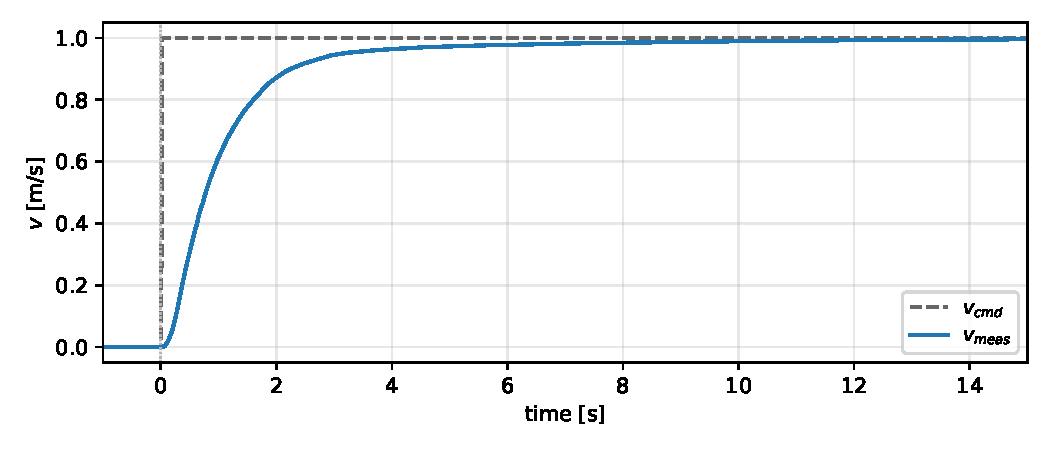
\includegraphics[width=0.9\linewidth]{figures/pid_step_surge.pdf}
\caption{Isolated surge velocity step response ($v_{\text{cmd}}:0\to1.0$~m/s, $w_{\text{cmd}}=0$): fused-odometry $v_{\text{meas}}(t)$ against the commanded step. The response is essentially first-order with no overshoot ($\sim$2\,s rise, $\sim$6.5\,s settling to the 2\% band).}
\label{fig:step_surge}
\end{figure}

\begin{figure}[H]
\centering
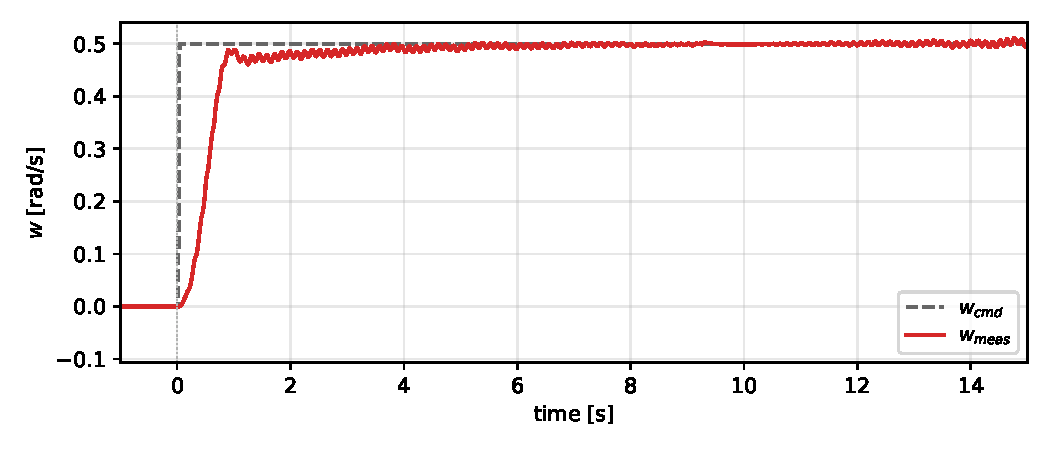
\includegraphics[width=0.9\linewidth]{figures/pid_step_yaw.pdf}
\caption{Isolated yaw-rate step response ($w_{\text{cmd}}:0\to0.5$~rad/s, $v_{\text{cmd}}=0$): $w_{\text{meas}}(t)$ against the commanded step. The yaw loop is markedly faster than surge ($\sim$0.5\,s rise) with a small $\sim$2\% overshoot and negligible steady-state error.}
\label{fig:step_yaw}
\end{figure}

\begin{figure}[H]
\centering
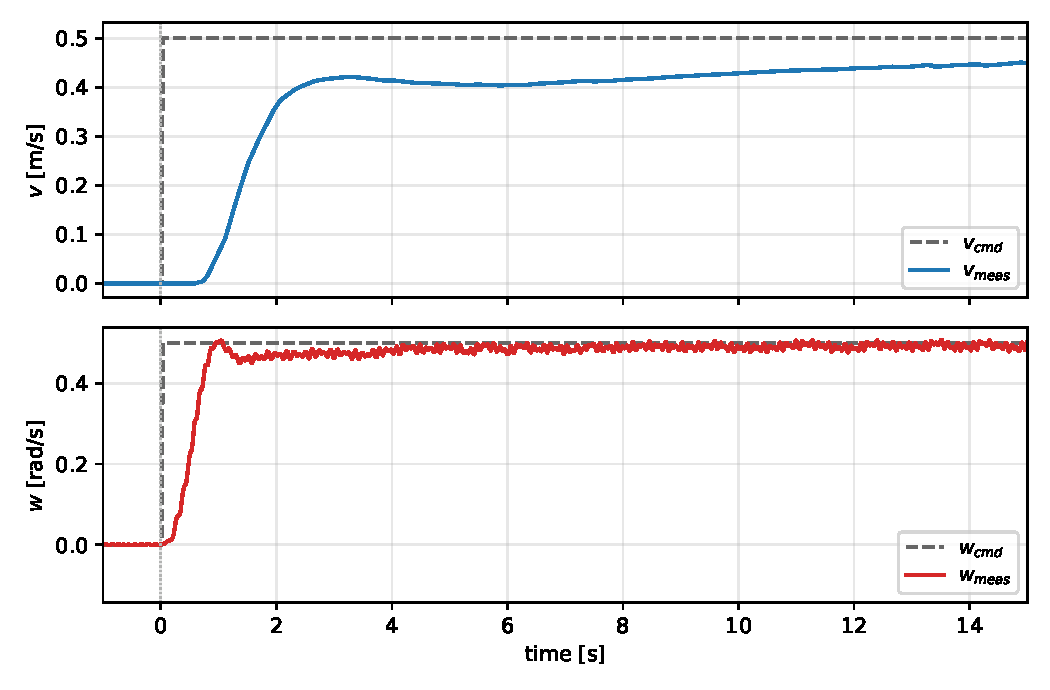
\includegraphics[width=0.9\linewidth]{figures/pid_step_coupled.pdf}
\caption{Coupled step ($v_{\text{cmd}}:0\to0.5$~m/s and $w_{\text{cmd}}:0\to0.5$~rad/s applied together). Yaw tracking (bottom) is essentially unaffected, but surge (top) becomes sluggish and settles $\sim$10\% low: with both a common-mode (surge) and a differential (yaw) thrust demand, one thruster approaches its $\pm T_{\max}$ limit and surge authority is transiently sacrificed to preserve yaw.}
\label{fig:step_coupled}
\end{figure}

\begin{table}[H]
\centering
\caption{Velocity-tracking performance metrics, isolated surge and yaw step tests (Gazebo, simulation gains).}
\label{tab:vwresults}
\begin{tabular}{@{}lcccc@{}}
\toprule
Axis & Rise time (10--90\%) & Overshoot [\%] & Settling time (2\%) & Steady-state error\\
\midrule
Surge $v$ ($0\to1.0$~m/s)  & 2.0\,s & 0.0 & 6.5\,s & $\approx 0.004$~m/s \\
Yaw $w$ ($0\to0.5$~rad/s)  & 0.5\,s & 2.2 & 4.3\,s & $\approx 0.001$~rad/s \\
\bottomrule
\end{tabular}
\end{table}

Both axes track their setpoints with negligible steady-state error, confirming that the integral action (with directional anti-windup, Section~\ref{sec:pid}) removes the residual drag offset. The yaw loop is roughly four times faster than surge, consistent with its much higher proportional gain (Table~\ref{tab:pid}). The coupled test (Figure~\ref{fig:step_coupled}) shows the decoupling assumption holds well for yaw but only approximately for surge under simultaneous large yaw demand, where thruster saturation in the mixer (Eqs.~\eqref{eq:mixL}--\eqref{eq:mixR}) reduces available surge force.

\subsection{Trajectory-following performance}

\textbf{Test protocol.} The full ILOS guidance stack (Section~\ref{sec:ilos}) was run in the Gazebo digital twin on a closed \emph{square} mission: a $40\times40$~m box (waypoints offset $3$~m in East from the spawn point) traversed for $3$ consecutive laps, using the square-mission guidance parameters of Table~\ref{tab:ilosparams} ($k_i=0$, i.e.\ pure LOS, in calm water with no current). The vehicle pose was logged at the $10$~Hz guidance rate; cross-track error $e_y$ and the per-lap/per-leg statistics were computed online by the characterization node.

\begin{figure}[H]
\centering
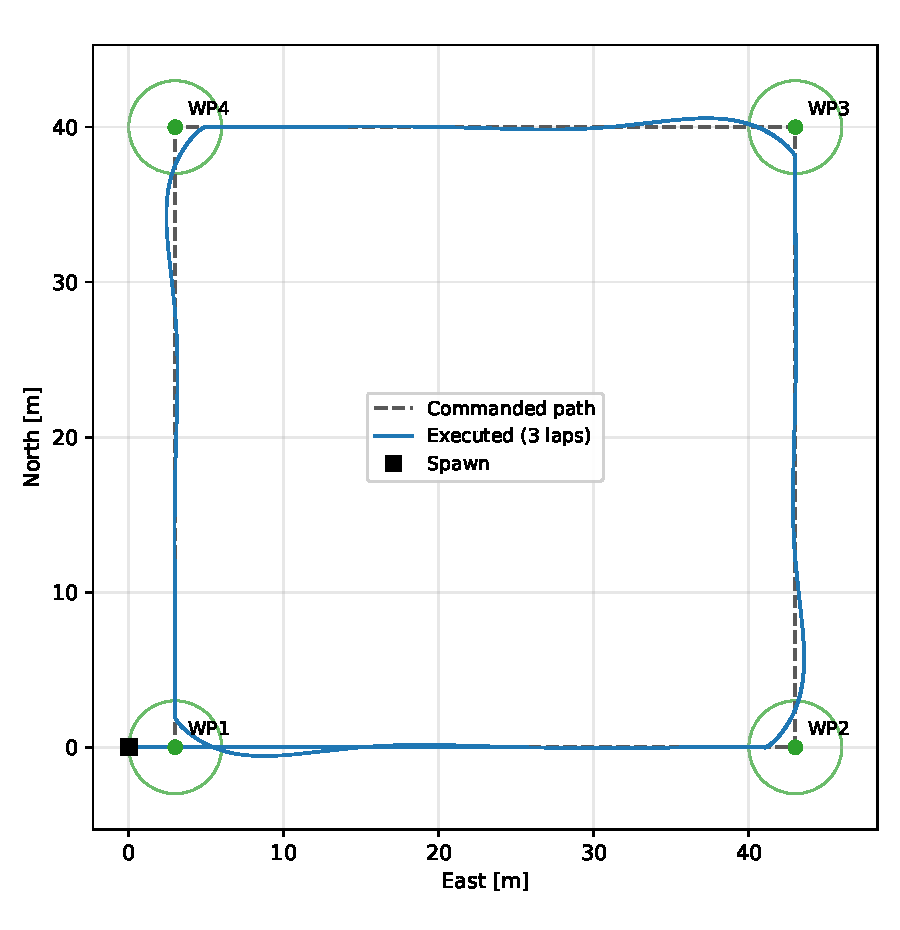
\includegraphics[width=0.72\linewidth]{figures/traj_square_path.pdf}
\caption{Executed path (ENU) over 3 laps against the commanded square. Waypoint markers show the $R_{\text{wp}}=3$~m arrival radius; the vehicle deliberately cuts each corner as it switches to the next leg once inside $R_{\text{wp}}$, so the executed path ($429$~m) is shorter than the ideal polyline ($480$~m).}
\label{fig:traj_path}
\end{figure}

\begin{figure}[H]
\centering
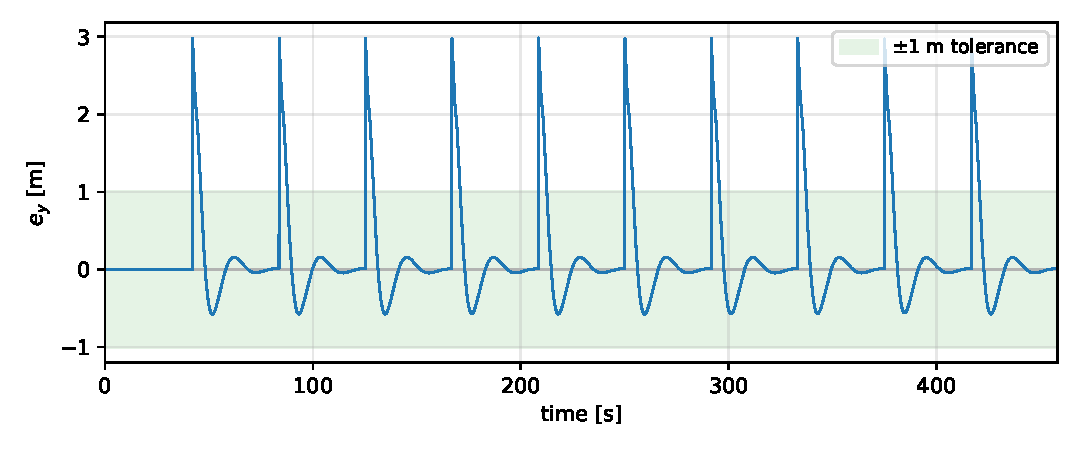
\includegraphics[width=\linewidth]{figures/traj_square_ey.pdf}
\caption{Cross-track error $e_y(t)$ for the square mission. On the straight legs $e_y$ is held to the millimetre level; each of the 11 corners produces a transient spike to $\sim$3~m (the vehicle is momentarily off the \emph{new} leg the instant it switches at the waypoint), which the LOS law rejects within a few seconds with a small ($\sim$0.7~m) undershoot before re-converging. The shaded band is the $\pm1$~m tolerance used for the coverage metric.}
\label{fig:traj_ey}
\end{figure}

\begin{table}[H]
\centering
\caption{Trajectory-following performance metrics, square mission (Gazebo, 3 laps, $k_i=0$).}
\label{tab:ilosresults}
\begin{tabular}{@{}lc@{}}
\toprule
Metric & Square mission \\
\midrule
Mean cross-track error $|e_y|$ & 0.29~m \\
RMS cross-track error $e_y$ & 0.64~m \\
Max $|e_y|$ (at corners) & 2.98~m \\
Fraction of path within $\pm1$~m & 91.4\% \\
Mean waypoint closest approach & 2.99~m ($\approx R_{\text{wp}}$) \\
Total mission time (3 laps) & 458~s \\
Executed / ideal path length & 429~m / 480~m \\
\bottomrule
\end{tabular}
\end{table}

The tracking behaviour is dominated by the waypoint transitions: away from the corners the pure-LOS law holds the vehicle essentially on the line ($91.4\%$ of the path lies within $\pm1$~m), and the entire $0.64$~m RMS budget is accumulated in the brief post-corner transients visible in Figure~\ref{fig:traj_ey}. The mean waypoint closest approach ($2.99$~m) simply reflects the $R_{\text{wp}}=3$~m switching radius rather than a tracking deficiency -- the vehicle intentionally rounds each corner. The three laps are highly repeatable (per-lap RMS $e_y$ within $0.55$--$0.67$~m), confirming the guidance law reaches a consistent steady cornering pattern.

\subsection{Discussion}

\todored{Once the above tables/figures are filled in: (1) comment on whether the simulation-derived PID gains (Table~\ref{tab:pid}) transferred acceptably to the real vehicle or needed re-tuning; (2) comment on whether $k_i=0$ (ILOS integral disabled, Table~\ref{tab:ilosparams}) was sufficient given observed cross-track error, or whether enabling the integral term is recommended for future missions; (3) note any observed thruster saturation, RC-override events, or GPS/EKF glitches that affected the results.}

% =============================================================================
\section*{Conclusion}
% =============================================================================
\addcontentsline{toc}{section}{Conclusion}

This report described the full autonomy stack of the \textit{Lily} ASV: its physical/sensing configuration and IMU/GPS-fused localization, an in-water-calibrated propulsion chain from commanded thrust to FOC-driven ERPM, a decoupled, relay-autotuned surge/yaw PID velocity controller with thruster mixing, an Integral-LOS trajectory-following law, and a GPS-waypoint mission-management FSM that sequences trajectories from a series of waypoints, together with a Gazebo-based digital twin used for development and validation. \todored{Close with 2--3 sentences summarizing the actual quantitative results once Section~\ref{sec:results} is filled in.}


\end{document}
